\newpage
\chapter{Общие свойства одномерного движения}
\par 1\textdegree. Если $U=U_1(x)+U_2(y)+U_3(z)$, то $\psi=\psi_1(x)\psi_2(y)\psi_3(z)$, т.е. для каждой из этих функций получим одномерную задачу.
\par 2\textdegree. \begin{theorem} Для одномерного случая все уровни дискретного спектра не вырождены.
\end{theorem}
\par \proof Пусть есть $\psi_1$ и $\psi_2$, соответствующие одному значению энергии E. Тогда из УШ получим
$$\frac{\psi_1^\prime\prime}{\psi_1} = \frac{2m}{\hbar^2}(U-E)=\frac{\psi_2^\prime\prime}{\psi_2}$$
\par Тогда $ \psi_1^\prime\prime\psi_2 - \psi_1 \psi_2^\prime\prime=0$. Запишем в виде полной производной и проинтегрируем: $\psi_1^\prime\psi_2 - \psi_1 \psi_2^\prime=const$. Рассмотрим предел $x \rightarrow \infty$: $\psi_{1,2} \rightarrow 0$. Т.к. состояние связанное (спектр дискретный), то $const \equiv 0$. Что из этого следует: $ \frac{\psi_1^\prime}{\psi_1} = \frac{\psi_2^\prime}{\psi_2}$ и $\psi_1 = const \cdot \psi_2 $.
\textbf{Теорема доказана}
\par 3\textdegree.\begin{theorem} \textbf{Осцилляционная теорема} Любая собственная функция $\psi_n$, соответствующая собственному значению $E_{n+1}$, обращается в нуль n раз (при конечных х).\end{theorem}
\par \proof \par Доказательство давал Антон Андреевич, оно под звездочкой, будет время - включим в документ. \textbf{Теорема доказана}
\par 4\textdegree. Классификация спектра.
\par \begin{wrapfigure}[10]{r}{0.5\linewidth} 
\vspace{-2ex}
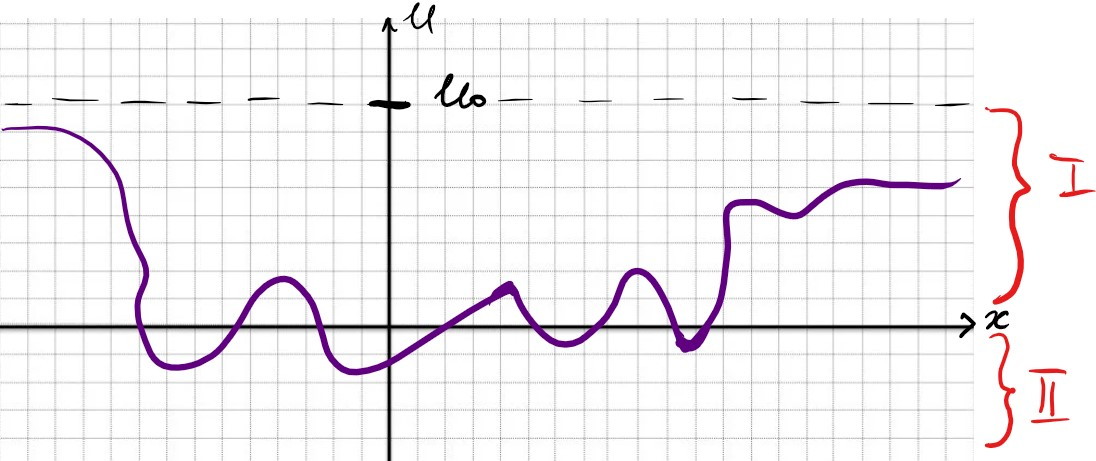
\includegraphics[width=1\linewidth]{pictures/20.1.jpg}
\caption{Классификация спектра}
\end{wrapfigure}
\par Область I на рисунке соответствует непрерывному спектру, но собственные значения $E_n$ не вырождены. Область II: $E<U$ асимптотически, спектр дискретный, в системе наблюдается затухание.
$$k=\sqrt{\frac{2mE}{\hbar^2}}$$
//много слов, есть парочка формул//
\par $\psi \rightarrow^{x \rightarrow \infty} a cos(kx+\delta) $, где $\delta$  - фаза рассеяния. Т.к. потока на бесконечности нет, там стенка потенциала (косинус выбрали, т.к. амплитуда упавшей и отраженной от стенки волн должны быть одинаковы).
\par При $x \rightarrow -\infty$ получим 
$$\psi\prime\prime - \frac{2m}{\hbar^2}(U_0 - E)\psi =0$$
\par Тогда $\psi = b e^{\kappa x}$, $\kappa = \frac{1}{\hbar}\sqrt{2m(U_0-E)}$ - затухание.
\par В неотмеченной области $E>U_0$ спектр непрерывный, но все уровни двухкратно вырождены. Оба независимых решения на бесконечностях удовлетворяют хорошим ГУ.
\par 5\textdegree. Если потенциал $U(x)$ - четная функция, то мы можем определить четность волновой функции. Итак, $\psi(x)$ - решение УШ
$$\hat{H}(x)\psi(x)=E\psi(x)$$
\par Сменим х на -х в этом уравнении
$$\hat{H}(-x)\psi(-x)=E\psi(-x)$$
\par Т.к. потенциал - функция четная, как и $\frac{\partial^2}{\partial x^2}$, то оператор Гамильтона не изменится, тогда $\psi(-x)$ - тоже решение УШ
$$\hat{H}(x)\psi(-x)=E\psi(-x)$$

\par Можем тогда сказать, что $\psi(-x)=C \psi(x)$, а если еще раз сменить -х на х, то получим еще одну связь $\psi(x)=C^2\psi(x)$ и константа $C=\pm 1$. Значит, \textit{все решенич есть четные или нечетные функции} и симметрия решения всегда меньше симметрии уравнения. Для основного состояния $\psi$-функция четная.

//+добавить этот же кусок в билет про четность состояния//
\par 6\textdegree. Нормировочный коэффициент непрерывного спектра
\par \textbf{a)} Рассмотрим волновую функция для движения, инфинитного в одну сторону $x \rightarrow \infty $. Нормировочный интеграл расходится на бесконечности, и это основной вклад в интеграл. Левый предел интегрирования можно выбрать любым образом. Пусть, например, x=0
$$\int \psi^*_p \psi_{p^\prime}dx = \delta \left( \frac{p-p^\prime}{2\pi \hbar}\right)$$
\par где р - импульс на бесконечности. При $x \rightarrow \infty$ имеем $\psi_p \approx  2 cos(kx+\delta)= e^{-i(kx+\delta)}+e^{i(kx+\delta)}$ - 2 стоячие волны. $p \rightarrow p\prime$, выкинем слагаемые с суммой $k$ и $k^\prime$, т.к. они не дадут $\delta$-функцию:
$$\int \psi^*_p \psi_{p^\prime}dx = \int^{\infty}_0 e^{i(k^\prime-k)x} dx + \int^{\infty}_0 e^{-i(k^\prime-k)x} dx = \int^{\infty}_{\infty} e^{i(k^\prime-k)x} dx $$
\par \textbf{б)} Переход к нормировке на $\delta$-функцию по энергии. Учтем в $\psi_p$:
$$\frac{d \left(\frac{p}{2\pi\hbar} \right)}{dE}^{\frac{1}{2}} = \frac{1}{\sqrt{2\pi\hbar V}} $$
$$\psi_E= \frac{\psi_p}{\sqrt{2\pi\hbar V}} = \frac{1}{\sqrt{2\pi\hbar V}} \left(e^{-i(kx+\delta)}+e^{i(kx+\delta)} \right)$$